% --- SAM 1, SAM 2, and SAM 3 ---
\begin{frame}{Segment Anything Model (SAM): A foundation model targeted for segmentation}
  \centering
  
\includegraphics[width=\textwidth,height=0.86\textheight,keepaspectratio]{assets/New-Lecture_Foundation_models/stanford_biods276_lecture1/slide_27.png}
\end{frame}

\begin{frame}{Segment Anything Model (SAM): A foundation model targeted for segmentation}
  \centering
  
\includegraphics[width=\textwidth,height=0.86\textheight,keepaspectratio]{assets/New-Lecture_Foundation_models/stanford_biods276_lecture1/slide_28.png}
\end{frame}



\begin{frame}{How does SAM work?}
  \begin{itemize}
    \item Encodes images into embeddings using a transformer backbone.
    \item User or downstream model provides prompts (points, boxes, text).
    \item The model predicts segmentation masks accordingly.
    \item Produces high-quality object masks across a wide range of settings without the need for fine-tuning.
  \end{itemize}
  \centering
  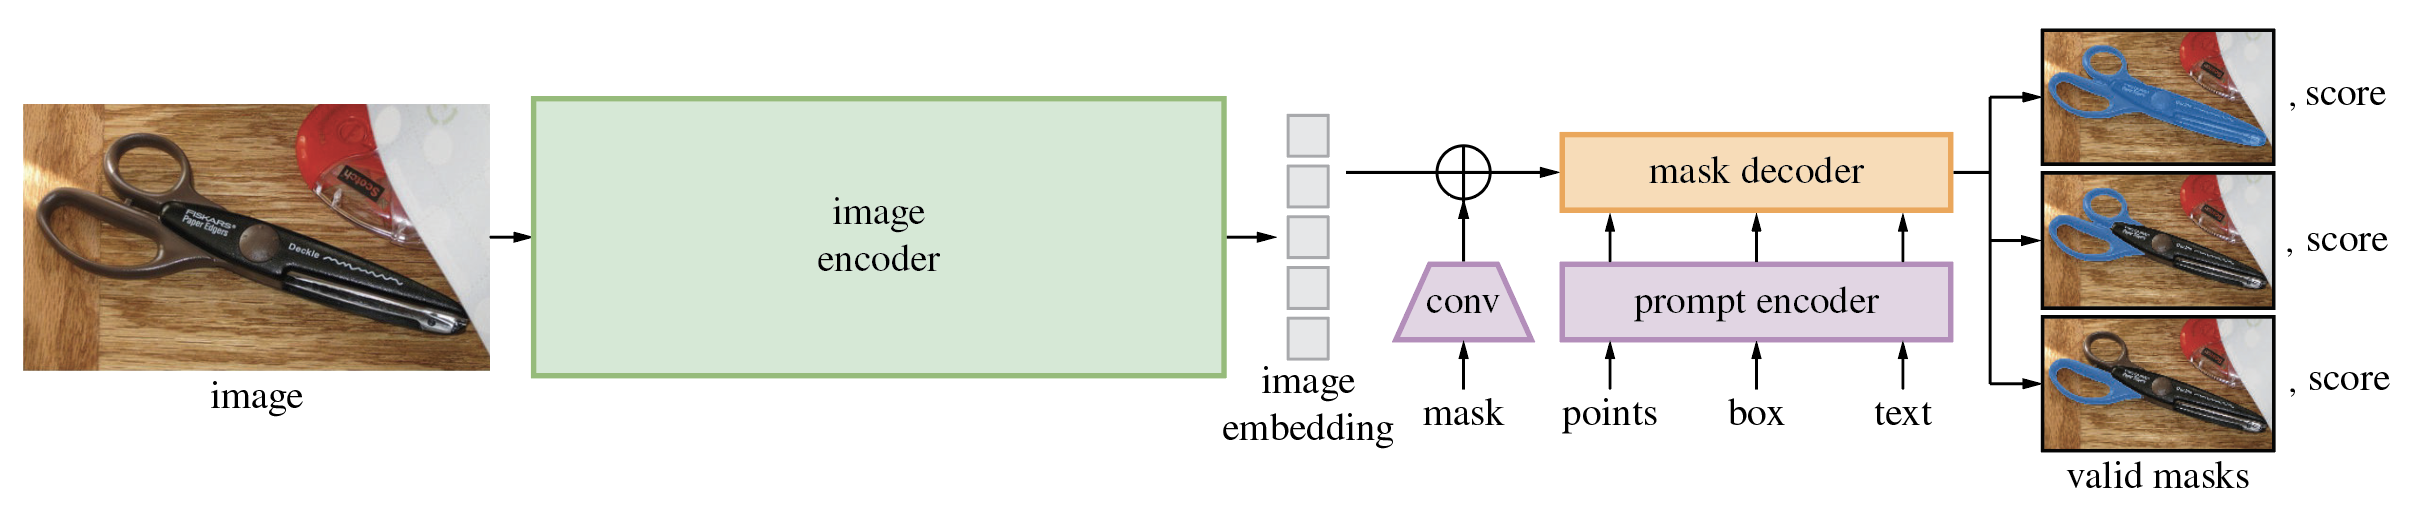
\includegraphics[width=0.85\textwidth]{assets/New-Lecture_Foundation_models/sam_schema.png}
\end{frame}

\begin{frame}{SAM 1, SAM 2, and SAM 3: What’s the Difference?}
  \begin{columns}[T,onlytextwidth]
    \begin{column}{0.32\textwidth}
      \textbf{SAM 1}
      \begin{itemize}\footnotesize
        \item Segments any object in any image.
        \item Requires as little as a single click to segment an object.
        \item Refine prediction with a few clicks.
      \end{itemize}
    \end{column}
    \begin{column}{0.32\textwidth}
      \textbf{SAM 2}
      \begin{itemize}\footnotesize
        \item Segments and tracks any object in any image or video.
        \item Uses click, box, or mask prompts.
        \item Tracks segment predictions across video frames.
        \item Refine prediction with a few clicks.
      \end{itemize}
    \end{column}
    \begin{column}{0.32\textwidth}
      \textbf{SAM 3}
      \begin{itemize}\footnotesize
        \item Detect, segment and track every example of any object category in image or video.
        \item Uses text or examples as prompts.
        \item Segments and tracks objects from a click.
        \item Tracks segment predictions across frames.
        \item Detects and segments matching instances.
        \item Refine detection with visual examples.
      \end{itemize}
    \end{column}
  \end{columns}
\end{frame}


\begin{frame}{SAM 3 Architecture: Data Engine}
  \centering
  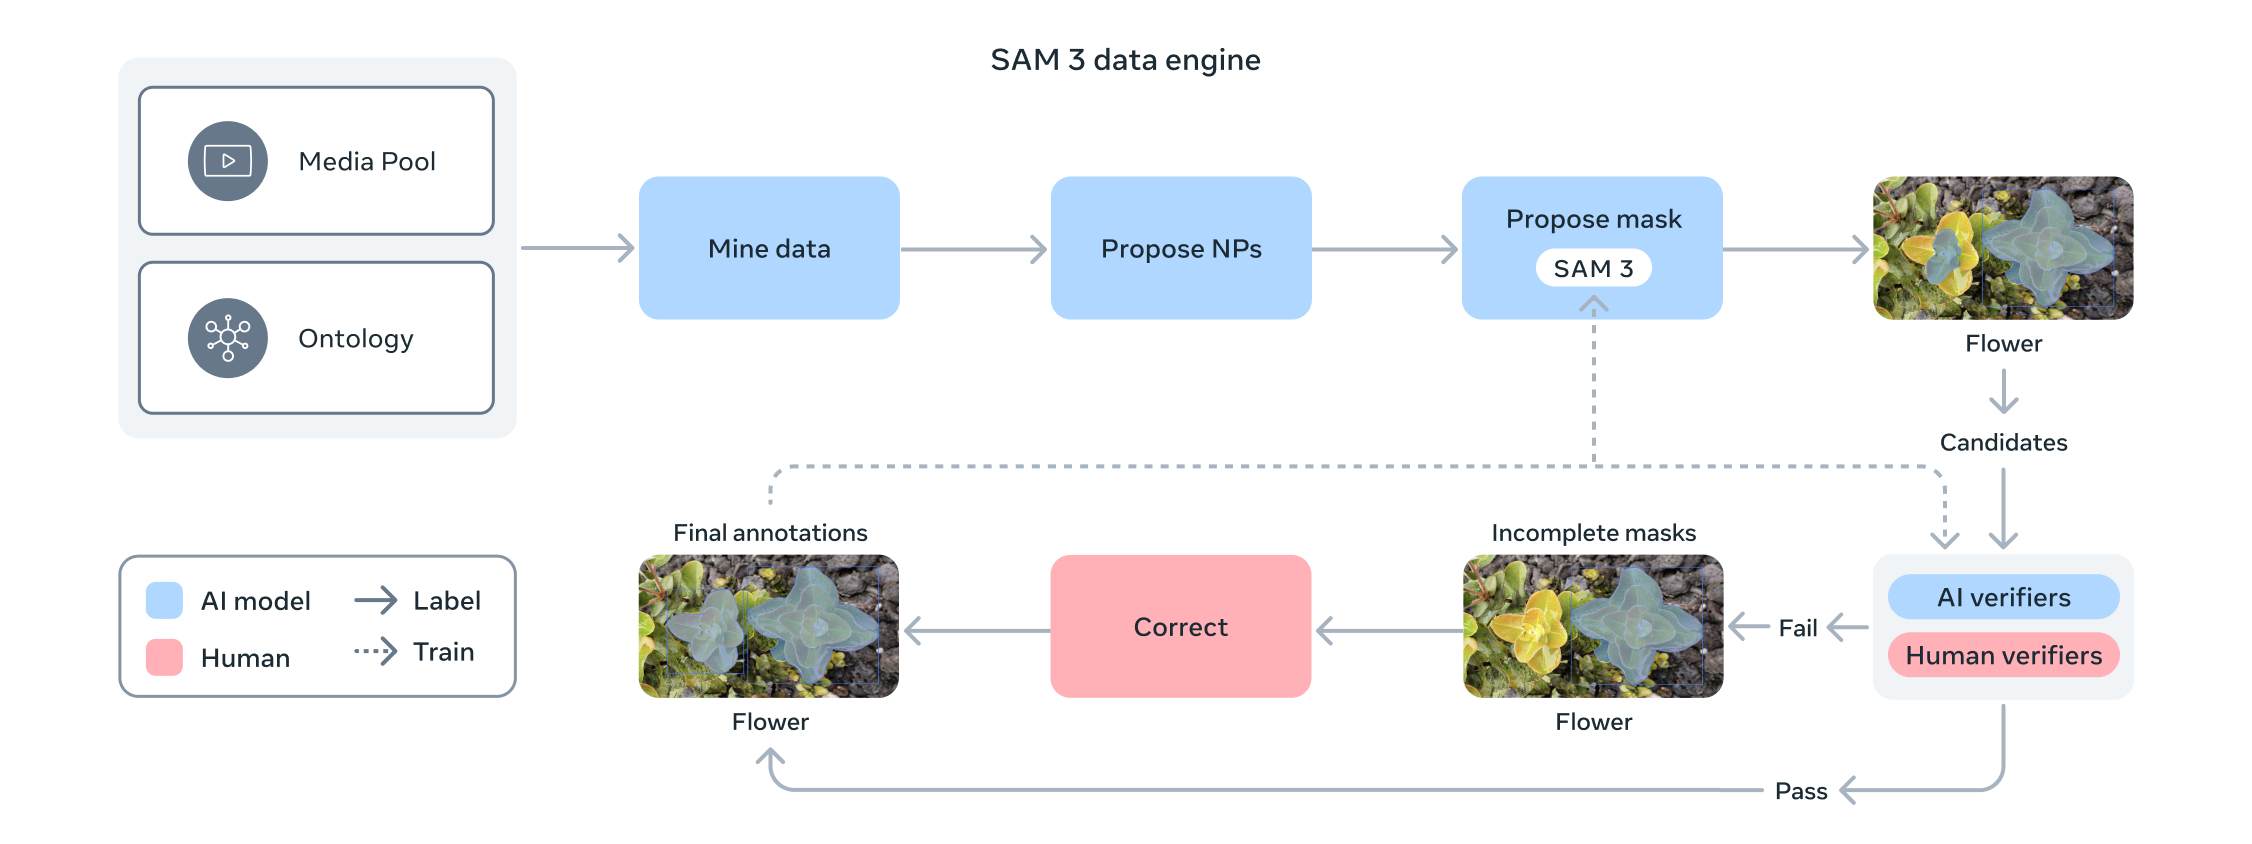
\includegraphics[width=0.82\textwidth, height=0.86\textheight, keepaspectratio]{assets/New-Lecture_Foundation_models/sam3_blog/sam3_blog_img_10.png}\\[0.1em]
  {\scriptsize SAM 3 data-engine loop from Meta blog post.}
  \vspace{0.5em}
  \begin{itemize}\footnotesize
    \item Obtaining high-quality annotated images with segmentation masks and text labels across a broad range of categories and visual domains is a significant challenge. A scalable data engine combining SAM 3, human annotators, and AI models produced 4M+ high-quality, annotated concepts across diverse domains.
    \item SAM 3 uses a scalable data engine where AI models and annotators (human and Llama-based) collaborate in a feedback loop to rapidly mine, annotate, and verify segmentation datasets—significantly increasing throughput and data quality.
  \end{itemize}
\end{frame}


\begin{frame}{SAM 3 Architecture: Core Model}
  \centering
  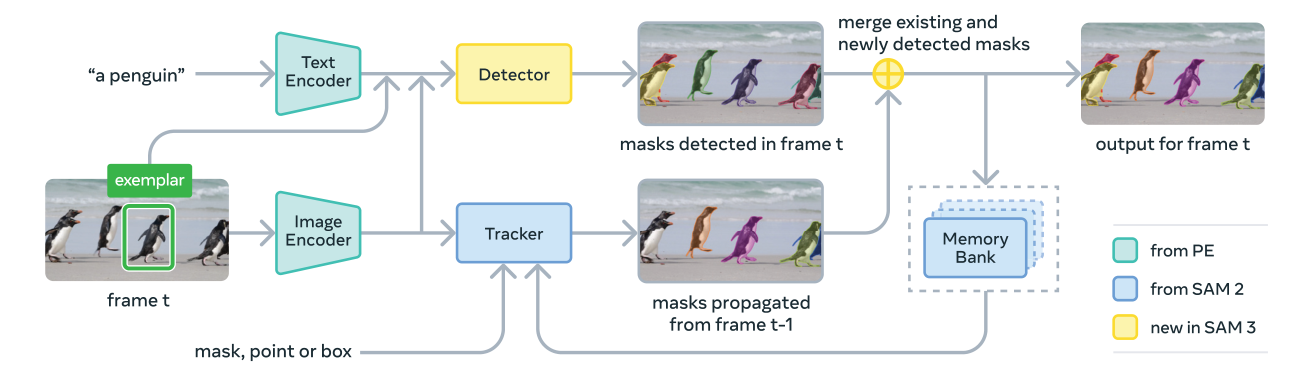
\includegraphics[width=0.82\textwidth, height=0.86\textheight, keepaspectratio]{assets/New-Lecture_Foundation_models/sam3_paper/sam3_page4_architecture_overview.png}\\[0.15em]
  {\scriptsize SAM 3 model summary and detector/tracker architecture.}
  \break
  \footnotesize
  Dual encoder-decoder transformer—serving as a detector for image-level capabilities—used together with a tracker and memory for video. The detector and tracker both receive vision-language features from an aligned Perception Encoder (PE) backbone.
\end{frame}


\begin{frame}{SAM 3.1 Inference Architecture: Object Multiplexing}
  \centering
  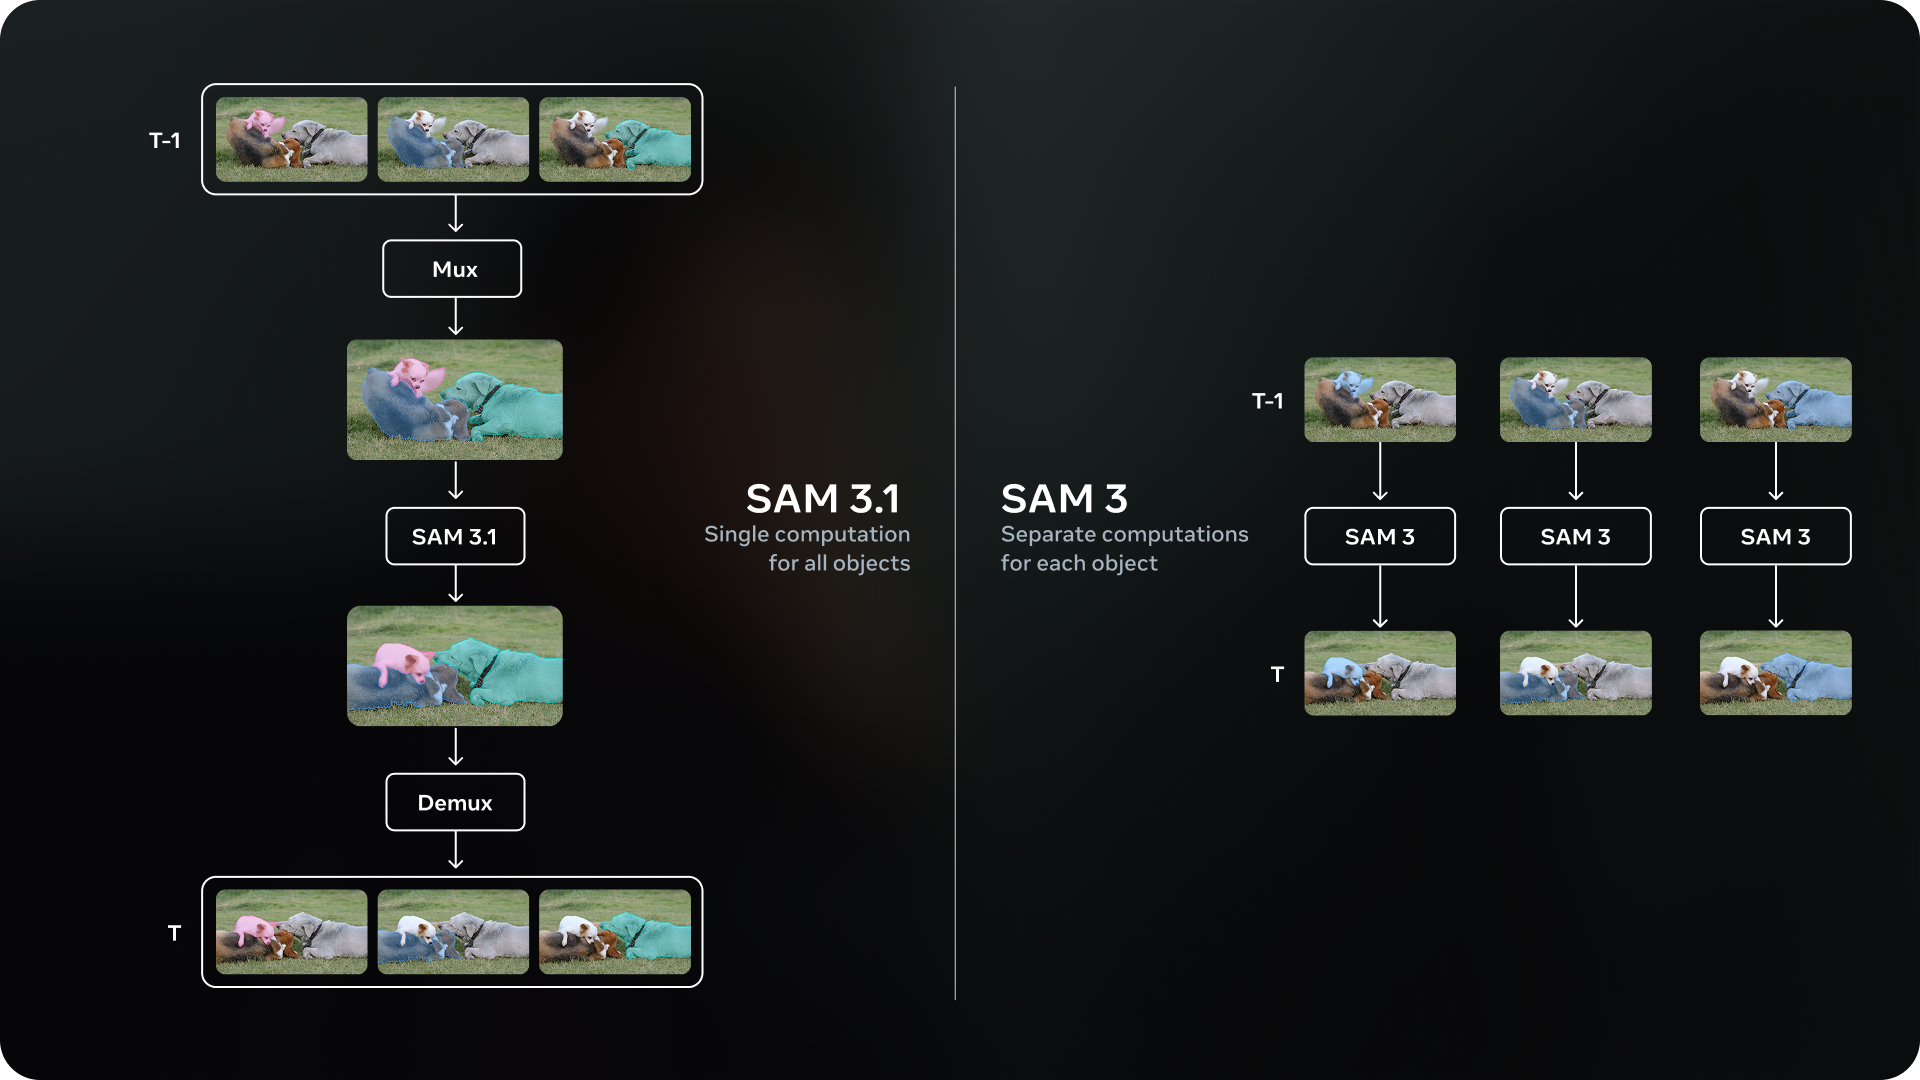
\includegraphics[width=0.75\textwidth, height=0.75\textheight, keepaspectratio]{assets/New-Lecture_Foundation_models/sam3_blog/sam3_blog_img_02.png}\\[0.1em]
  {\scriptsize SAM 3.1 multiplexed inference versus per-object computation.}
  \vspace{0.5em}
  \begin{itemize}\footnotesize
    \item Process multiple tracked objects in one forward pass (\emph{multiplexing}) instead of one pass per object.
    \item Shared object-level context reduces redundant compute and helps crowded-scene tracking.
  \end{itemize}
\end{frame}
